% This is a Homework Template for CS 1010.  
% It was modified by  Michael Carl Tschantz (mtschant) 
% who provided the ``useful infomation on latex''.

% THE ONLY THING YOU NEED TO DO IN THIS PART IS 
% TO FILL IN THE HOMEWORK NUMBER, YOUR NAME AND LOG IN BELOW
% REPLACE ``X'' WITH THE HW NUMBER, ``Your Name'' WITH YOUR NAME,
% AND ``your login'' WITH YOUR LOGIN.

\newcommand{\hwnumber}{12}
\newcommand{\yourname}{Michael Mueller}

% NOW YOU MAY SKIP DOWN TO THE PART CALLED ``YOUR DOCUMENT''.

%==============================================================================
% Formatting parameters (how the page is set up)
%==============================================================================
\newcommand{\yourcourse}{Math 695}
\newcommand{\chapter}{0}
\newcommand{\mgn}{\mathcal M_{g,n}}
\newcommand{\mgnb}{\overline{\mathcal M_{g,n}}}
\newcommand{\mgb}[1]{\overline{\mathcal M_{g,#1}}}

\documentclass[11pt]{article}           % 11pt article
\makeatletter                   % Make '@' accessible.
\pagestyle{myheadings}              % We do our own page headers.
\newcommand{\thishw}{\bf Elliptic curve question in deg 4}
\def\@oddhead{\bf \thishw \hfill \yourname}
\oddsidemargin=0in              % Left margin minus 1 inch.
\evensidemargin=0in             % Same for even-numbered pages.
\textwidth=6.5in                % Text width (8.5in - margins).
\topmargin=0in                  % Top margin minus 1 inch.
\headsep=0.2in                  % Distance from header to body.
\textheight=8in                 % Body height (incl. footnotes)
\skip\footins=4ex               % Space above first footnote.
\hbadness=10000                 % No "underfull hbox" messages.
\makeatother                    % Make '@' special again.

%==============================================================================
% Packages used (packages add more commands)
%==============================================================================

\usepackage{amsmath}                % give more fonts and symbols
\usepackage{amsfonts}               % want AMS fonts
\usepackage{amssymb}
\usepackage{amsthm}
\usepackage{mathrsfs}
\usepackage{tikz-cd}
\usepackage{bbm}                % given mathbbm fonts
\usepackage[shortlabels]{enumitem}
\usepackage{relsize}
\usepackage{hyperref}

\makeatletter
\newcommand*{\relrelbarsep}{.386ex}
\newcommand*{\relrelbar}{%
  \mathrel{%
    \mathpalette\@relrelbar\relrelbarsep
  }%
}
\newcommand*{\@relrelbar}[2]{%
  \raise#2\hbox to 0pt{$\m@th#1\relbar$\hss}%
  \lower#2\hbox{$\m@th#1\relbar$}%
}
\providecommand*{\rightrightarrowsfill@}{%
  \arrowfill@\relrelbar\relrelbar\rightrightarrows
}
\providecommand*{\leftleftarrowsfill@}{%
  \arrowfill@\leftleftarrows\relrelbar\relrelbar
}
\providecommand*{\xrightrightarrows}[2][]{%
  \ext@arrow 0359\rightrightarrowsfill@{#1}{#2}%
}
\providecommand*{\xleftleftarrows}[2][]{%
  \ext@arrow 3095\leftleftarrowsfill@{#1}{#2}%
}
\makeatother

%==============================================================================
% Macros (make your own commands)
%==============================================================================

% For problem and part headers
\newcounter{problemcounter}
\newcounter{subproblemcounter}
\newcommand{\problem}{
    \addtocounter{problemcounter}{1}
    \bigskip
    \noindent {\Large Problem \hwnumber .\theproblemcounter}
    \smallskip
    \setcounter{subproblemcounter}{0}
}
\newcommand{\subproblem}{
    \addtocounter{subproblemcounter}{1}
    \smallskip
    \noindent {\bf \alph{subproblemcounter})} 
}

% Nice things
\newcommand{\set}[1]{\{#1\}}            % Set (as in \set{1,2,3})
\newcommand{\setof}[2]{\{\,{#1}|~{#2}\,\}}  % Set (as in \setof{x}{x > 0})

% Some letter symbols
\newcommand{\N}{\ensuremath{\mathbb{N}}}
\newcommand{\Z}{\ensuremath{\mathbb{Z}}}
\newcommand{\R}{\ensuremath{\mathbb{R}}}
\newcommand{\hTop}{\textbf{hTop}}
\newtheorem*{Proposition}{Proposition}
\newtheorem*{Corollary}{Corollary}
\newcommand{\Tor}{\text{Tor}}
\newcommand{\Ext}{\text{Ext}}
\newcommand{\Q}{\mathbb{Q}}
\newcommand{\F}{\mathbb{F}}
\newcommand{\C}{\mathbb{C}}
\newcommand{\CP}{\mathbb{CP}}
\newcommand{\RP}{\mathbb{RP}}
\newcommand{\Spec}{\text{Spec}}
\newcommand{\Aut}{\text{Aut}}
\newcommand{\Proj}{\text{Proj}}
\newcommand{\Mor}{\text{Mor}}
\newcommand{\codim}{\text{codim}}
\newcommand{\exer}[1]{{\bf Exercise #1} \\}
\newcommand{\Hom}{\text{Hom}}
\newcommand{\coker}{\text{coker}}
\newcommand*\simplex{\includegraphics[scale=0.017]{simplex.png}}
\newcommand{\Sch}{\textbf{Sch}}
\newcommand{\Set}{\textbf{Set}}
\renewcommand{\P}{\mathbb P}
\theoremstyle{definition}
\newtheorem*{thm}{Theorem}
\newtheorem*{prob}{Problem}
\newtheorem*{dfn}{Definition}
\newtheorem*{claim}{Claim}
\theoremstyle{definition}
\newtheorem*{lem}{Lemma}
\newtheorem*{ex}{Exercise}
\newtheorem*{eg}{Example}
\newtheorem*{note}{Note}

%==============================================================================
% YOUR DOCUMENT (start here)
%==============================================================================

\begin{document}
\centerline{\LARGE\thishw}
\begin{prob}
  Let $(E,p_1,\dots,p_n)$ be a genus 1 curve with distinct marked points $p_1,\dots,p_n$. Let $\mu_0,\mu_1,\dots,\mu_{n+2}$ be partitions of an integer $d$ with $|\mu_0|=n$.

  How many maps $f:(E,p_1,\dots,p_n)\to (\P^1,0)$ are there (up to isomorphism) such that $f$ has ramification profile $\mu_0$ over $0$ corresponding to the
  points $p_1,\dots,p_n$ and ramification profiles $\mu_1,\dots,\mu_{n+2}$ over $n+2$ other unspecified points of $\P^1$? Let $X$ be the set of maps $E\to \mathbb P^1$ of this form;
  we will be interested in studying the numbers
  \[N_{\mu_0,\mu_1,\dots,\mu_{n+2}}=\#\frac{X}{\Aut(\P^1,0),\Aut(E,p_1,\dots,p_n)}\]
  where this is an orbifold count. (We require that $\mu_i\neq (1,1,\dots,1)$ for $i>0$; TODO why?)
\end{prob}

\begin{eg}
  Consider the case where $d=2$, $n=1$ and $\mu_0=\mu_1=\mu_2=\mu_3=(2)$.
  We know that there is a unique map $(E,p)\to (\mathbb P^1,0)$ of the specified form
  up to automorphisms of $\P^1$, and it factors through the antipodal automorphism of $E$,
  so
  \[
  N_{(2),(2),(2),(2)}=\frac 12.
  \]
\end{eg}
\begin{eg}
  See ``gw\_orbifold.pdf'' for a proof that $N_{(2k),(2)^k,(2)^k,(2,1,1,\dots,1)}=\frac 32$ for $k>1$.
  \end{eg}

Let $d>2$. Up to automorphisms of $\P^1$, a degree $d$ map $f:E\to\P^1$ corresponds to a degree $d$ line bundle $\mathcal L$ and a basepoint-free two-dimensional subspace $V\subset H^0(\mathcal L)$. By Riemann-Roch, $\mathcal L$ gives an embedding $E\hookrightarrow\P(H^0(\mathcal L))\cong\P^{d-1}$, and a basepoint-free two-dimensional subspace $V\subset H^0(\mathcal L)$ corresponds to a well-defined composition
\[
E\hookrightarrow \P(H^0(\mathcal L))=\P(V\oplus V^{\perp})\dashrightarrow\P(V)\cong\P^1
\]
For the composition to be well-defined, $E$ should not intersect $\P(V^{\perp})$, a codimension 2 subspace of $\P(H^0(\mathcal L))$. Each fiber of the rational map
$\P(V\oplus V^{\perp})\dashrightarrow\P(V)$ is a hyperplane containing $\P(V^{\perp})$, and so the fibers of the map $E\to\P^1$ correspond to intersections $H\cap E$ where $H$ is some hyperplane containing $\P(V^{\perp})$. Thus, $N_{\mu_0,\dots,\mu_{n+2}}$ can be determined by embedding $E$ in $\P^{d-1}$ via $\mathcal L=\mathcal O(\mu_{0,1}p_1+\dots+\mu_{0,n}p_n)$ and counting the number of codimension 2 subspaces $\P(V^{\perp})\subset \P^{d-1}$ such that (a) $\P(V^{\perp})\cap E=\emptyset$, (b) $\P(V^{\perp})\subset H_0$ where $H_0\cap E=\mu_{0,1}p_1+\dots+\mu_{0,n}p_n$, (c) $\P(V^{\perp})\subset H_i$ where $H_i\cap E$ has shape $\mu_i$, for $i=1,\dots,n$.

Note that if $\P(V^{\perp})$ is such a codimension 2 subspace corresponding to a map $f$, then $-\P(V^{\perp})$ (applying the involution on $E$, which extends to an automorphism of $\P(H^0(\mathcal L))$) is as well and corresponds to $x\mapsto f(-x)$.

\begin{eg}
  Let's compute $N_{(3),(3),(2,1),(2,1)}$. Embedding $E\hookrightarrow\P^2$ via $\mathcal L=\mathcal O(3p)$, we want to count the points $q\notin E$ such that
  $q\in\ell_0$ (the line at infinity) and $q\in\ell_1$, where $\ell_1\cap E=3r$ for some $r\neq p$ (we don't need to worry about the simple ramification, which
  is guaranteed). Since $q=\ell_0\cap\ell_1$ we just need to count lines $\ell_1$ with $\ell_1\cap E=3r$ for $r\neq p$; these are flex lines corresponding to nontrivial 3-torsion points, of which there are $3^2-1=8$. Precomposition with the involution of $E$ corresponds to replacing $q$ with $-q$, which corresponds to replacing the 3-torsion point with its inverse. Therefore,
  \[
  N_{(3),(3),(2,1),(2,1)}=\frac{8}{2}=4.
  \]
\end{eg}
\begin{eg}
  Let's compute $N_{(2,1),(3),(2,1),(2,1),(2,1)}$. If $\mathcal O(2p_1+p_2)=\mathcal O(3p_{\infty})$, then we can embed $E$ in $\P^2$ with $p_{\infty}$ as the point at infinity
  and let $\ell_0$ be a line such that $\ell_0\cap E=2p_1+p_2$. We want to count points $q\notin E$ with $q\in \ell_0$ and $q\in \ell_1$, where $\ell_1$ is a flex line. This again amounts to counting flex lines, so $N_{(2,1),(3),(2,1),(2,1),(2,1)}=3^2=9$.

  For similar reasons, $N_{(1,1,1),(3),(2,1),(2,1),(2,1),(2,1)}=9$.
\end{eg}

Another way to count $N_{\mu_0,\dots,\mu_{n+2}}$: note that $\{H:\P(V^{\perp})\subset H\}$ is a line in $\P(H^0(\mathcal L))^*$.
Let $X_{\mu}=\{H\in\P(H^0(\mathcal L))^*:H\cap E\text{ has shape }\mu\}$.
Counting the number of possibilities $\P(V^{\perp})$ amounts to counting lines $\ell\subset\P(H^0(\mathcal L))^*$ such that $H_0\in\ell$, $H_1,\dots,H_{n+2}\in\ell$ for distinct points $H_i\in X_{\mu_i}$, and $\P(V^{\perp})\cap E=H_0\cap H_1\cap E=\emptyset$ (if $n=1$, this is automatic).
Letting $\pi:\P^{d-1}\dashrightarrow \{\text{lines in $\P^{d-1}$ through $H_0$}\}=\P^{d-2}$ send $x$ to the line through $x$ and $H_0$, the idea is to count points in $\P^{d-2}$ whose fiber contains distinct points $H_i\in X_{\mu_i}$.

Now we move on to $d=4$, and embed $E$ in $\P^3$ via
$\mathcal L=\mathcal O(4p)$. We have a stratification of $(\P^3)^*$:

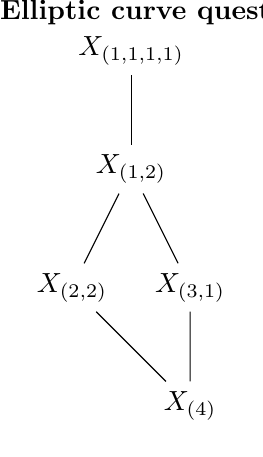
\begin{tikzpicture}
  \node {$X_{(1,1,1,1)}$}
  child {node {$X_{(1,2)}$}
    child {node[name=A] {$X_{(2,2)}$}}
    child {node {$X_{(3,1)}$}
      child {node[name=B] {$X_{(4)}$}}}};
  \draw (A) edge (B);
\end{tikzpicture}

First, note that \[X_{(2,2)}\cong\{(x,y)\in E^2:2x+2y=0\}=\{(x,y)\in E^2:x+y\text{ is 2-torsion}\}\]
so $X_{(2,2)}$ is a disjoint union of four curves each corresponding to a 2-torsion point $t_i$:
\[
C_i=\text{image}(f_i:E\hookrightarrow(\P^3)^*),\ f_i(x)=H\text{ where }H\cap E=2x+2(t_i-x)
\]
Note that $f_i$ is 2-to-1 ($x$ and $t_i-x$ are in the same fiber), so $C_i\cong E/S_2\cong\P^1$.

See ``Documents/four\_curves\_linear.m2'' for the computation in M2 to compute $X_{(2,2)}$; it turns out that each $C_i$ is a plane conic. By counting points of
intersection of the images of $C_i$ under $\pi:(\P^3)^*\dashrightarrow\P^2$, we find that
\[
N_{(4),(2,2),(2,2),(2,1,1)}=\frac 32
\]
as expected from the Hurwitz calculation. By changing $\pi$ (and therefore $H_0$), we can also find
\[
N_{(3,1),(2,2),(2,2),(2,1,1),(2,1,1)}=N_{(2,2),(2,2),(2,2),(2,1,1),(2,1,1)}=6,\]\[ N_{(2,1,1),(2,2),(2,2),(2,1,1),(2,1,1),(2,1,1)}=12,\ N_{(1,1,1,1),(2,2),(2,2),(2,1,1),(2,1,1),(2,1,1),(2,1,1)}=24
\]



\end{document}
